\chapter{Introduction to machine learning toolkits}
We have used two state-of-the-art toolkits in our project, to help us achieve our goals. These tools are:-
\begin{itemize}
    \item Intel OpenVINO Computer vision toolkit
    \item Tensor Virtual Machine (TVM)
\end{itemize}
Both these tools have the same high level goal, that being the deployment of pre-trained CNN models on different hardware platforms such as CPU, GPU , FPGA etc. thereby making the high level deep learning frameworks such as Tensorflow, Caffe etc. independent of the underlying hardware. However none of these tools alone can achieve our goals, making it necessary to use a combination of both, using certain components and features in each toolkit. Both Intel OpenVINO and TVM are described in detail in the next sections.  

\section{OpenVINO}


Intel OpenVINO is an open source toolkit from Intel that allows the deployment of pre-trained deep neural networks on different hardware platforms such as CPU, GPU, FPGA, etc. The toolkit is available for installation for the Windows operating system a
s well as selected Linux distributions. All of the tool's libraries and plugins except the FPGA plugin are a part of the open source GitHub repository.
The functionality of OpenVINO is divided among its components, Model Optimizer, Calibration Tool, Inference Engine. This is shown in figure \ref{fig:OpenVINO_workflow} and explained below. 
\begin{figure}[!hbpt]
    \centering
    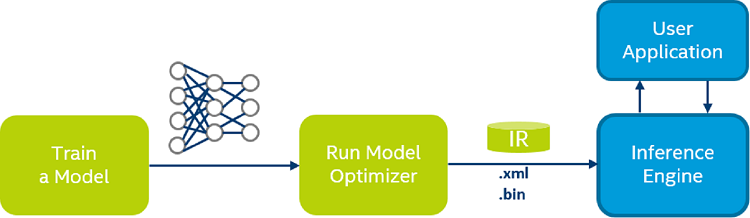
\includegraphics[width=0.65\textwidth]{img/openVINO_workflow.png}
    \caption{OpenVINO workflow \citep[cf.][]{openvino_fig}}
    \label{fig:OpenVINO_workflow}
\end{figure} 

\subsection{Model Optimizer}
The Model Optimizer is a python based tool which takes as input a pre-trained model. It supports many popular deep learning frameworks such as TensorFlow, Caffe, PyTorch, MXnet, etc. This model is then converted to a common intermediate format (IR), thereby making the inference engine independent of the training framework. The IR contains a .xml file which represents the computational graph of the CNN and a .bin file containing the weights. The graph is optimized by fusing different layers of the original topology wherever possible. Typically the batch normalization layers are fused with their preceding convolution layer and the convolution filter weights are accordingly adjusted. The toolkit comes with a model downloader which can download various openly available pre-trained models for different frameworks.
 

 \subsection{Inference Engine}
 The Inference Engine is responsible for the execution of the model on the selected hardware. For this purpose, it provides a C++ API which can be integrated into an application. The main task performed by the inference engine is to read the intermediate representation of the model, select the hardware for deployments such as CPU or FPGA and call the appropriate plugin which defines all necessary data structures and functions required to perform inference and return the output along with performance statistics. 
 The toolkit comes with pre-compiled bitstreams for a few supported FPGA boards. These bitstreams implement various popular network topologies such as GoogLeNet, ResNet, etc. as well as generic layers which are used to program the FPGAs as per the requirement of the given model topology.
 
 These bitstreams however, do not support the Intel Stratix 10 FPGA boards available in the noctua infrastructure. In addition to this, the FPGA plugin of the inference engine is not open source, making it infeasible to use OpenVINO as a stand alone tool to achieve our project goals without customizing its components at the source code level.
 
 \subsection{OpenVINO source code}
 The intel OpenVINO toolkit is open source and the code is available as a Github repository known as Deep Learning Deployment Toolkit (DLDT). The repository contains source code for both the Model Optimizer as well as the inference engine except for the FPGA plugin. As a result we have written our own FPGA plugin for OpenVINO with support for scaling over multiple FPGAs. 
 
 \subsection{FPGA plugin}
 The main purpose of the FPGA plugin is to flash the bitstreams (.aocx files) for the CNN models on the FPGAs and to launch the kernels according to the topology. It also supports scaling on multiple FPGAs which has been achieved through the use of MPI (Message Passing Interface) and the serial I/O channels present between FPGA nodes in the noctua infrastructure. 
 
 The plugin interacts with the inference engine C++ API which helps in parsing the intermediate representation obtained from the model optimizer for a given CNN model. We have reused the classes and data structures in this API as much as possible, specifically for parsing the .xml file in the IR containing the topology for the given CNN model, parsing the weights in the .bin file as well as parsing the input images.
 
 In addition to this pre-existing source code, we have written our own tree data structure in the plugin, to represent the CNN topology in a suitable pointer structure that adequately models the input output relationships between CNN layers, thus allowing us to launch their corresponding OpenCL kernels in an orderly fashion. 
 
 The plugin also supports scaling over multiple FPGAs, through the use of MPI and dedicated serial I/O connections between FPGA boards that are present in the noctua infrastructure. The infrastructure consists of 16 FPGA nodes, each hosting 2 Intel Stratix 10 FPGA boards. Our plugin has multiple instances running as MPI processes, one per node. Each plugin instance is thus responsible for the execution of partial CNN topology on 2 FPGAs. We divide the CNN model at the OpenCL level into multiple .cl files which are then synthesized to generate their corresponding bitstreams. These bitstreams are then named in a suitable fashion so as to create a mapping between them and the specific plugin instance running on a FPGA node which is identified by its MPI rank. To map the names of the CNN layers (OpenCL kernels) to the .aocx file that contains them, we use Intel OpenCL SDK binutils to generate a .xml file corresponding to each .aocx bitstream. The plugin instance would thus flash appropriate .aocx files according to its MPI rank and then launch appropriate kernels that are contained in those .aocx files, after parsing the corresponding xmls. 
 
 The sequence of operations take place during the execution of the plugin.
 
 \begin{itemize}
     \item The user application sends the CNN model IR and the input image to the plugin.
     \item The FPGA plugin parses the IR, both the xml and bin files to retrieve the layer information and the weights which are then used to construct a tree data structure.
     \item The plugin instance then flashes the appropriate bitstreams on the FPGA boards and parses their corresponding xml files to get a mapping between the aocx files and the kernel names.
     \item The kernels are then launched by a level wise traversal of the tree structure representing the CNN model.
     \item The plugin then collects results and returns them to the user application which displays the top N labels and their softmax scores (confidence) to the user.
 \end{itemize}
 
 \subsection{Advantages}
  
 \begin{itemize}
 \item Supports optimization of models and quantization of weights.
 \item A CNN model can be deployed on hardware with minimal programming effort and independent of the training framework.
 \item For FPGAs, the use of pre-compiled bitstreams eliminate the time needed for synthesis of kernel codes.
 \end{itemize}
 
 \subsection{Disadvantages}
 \begin{itemize}
 \item The main disadvantage is the compatibility of FPGA boards. Development and synthesis of kernel codes along with a plugin for FPGAs may be required to make OpenVINO work with unsupported boards. 
 \item Scaling to multiple FPGAs, which is one of the goals of this project is non-trivial as it would require the development of overlays for external I/O channels. 
 \end{itemize}
\section{TVM}

Today we have a lot of different deep learning frameworks such as TensorFlow, Caffe2, MXNet and PyTorch and hardware targets: CPUs, GPUs, FPGAs, and ASICs. During the mapping of one of the frameworks to a device, we run into the problem with a variety of hardware characteristics such as memory organization (implicitly managed, mixed, explicitly managed) and compute primitives (scalar, vector, tensor).

TVM takes the model from different learning frameworks and generates optimized code for devices. TVM was started as a research project at the Paul G. Allen School of Computer Science and Engineering, University of Washington.

TVM includes a computational graph rewriter, tensor expression language and new features for GPU accelerators. The TVM compilation stack is shown in Fig 5.2.

The system has the stack of implementation: NNVM $\to$ TOPI $\to$ TVM $\to$ VTA. Neural Network Virtual Machine (NNVM) acts as a graph optimizer by taking the model from an existing framework and converting it into “TVM” graph. For these operations, we use the TVM Operator Inventory (TOPI) language. TOPI is a library where functions operate as instructions for further work. For example, TOPI defines a tensor computation, schedules space for each NN operator (e.g. conv2d). The next step is the application of the TVM functions. TVM uses the TOPI instructions and generates code for several backends, such as Low Level Virtual Machine (LLVM), or Compute Unified Device Architecture (CUDA), etc. The final step is the Versatile Tensor Accelerator (VTA) which is responsible for the stream and microkernels. 

In order to change a hardware target ( CPU, GPU or TPU) we need to rebuild TVM libraries again.  

\begin{figure}[h!]
    \centering
    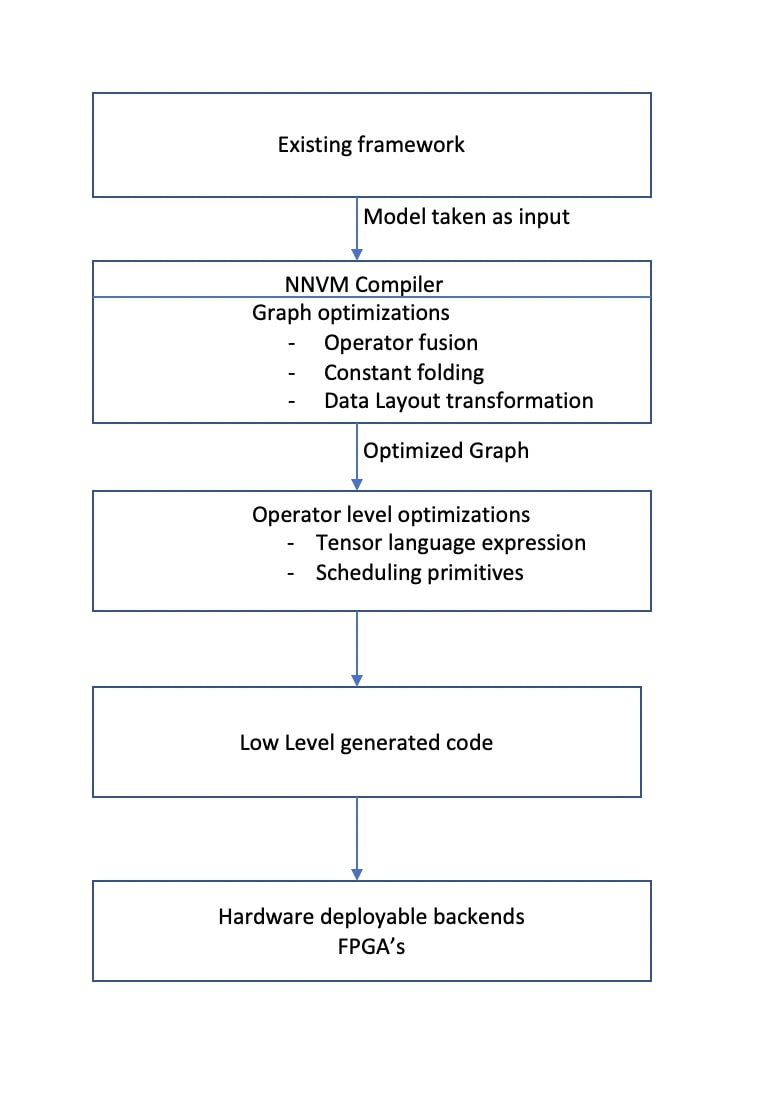
\includegraphics[scale=0.30]{TVM.png}
    \caption{TVM Flowchart}
\end{figure}
 
 \subsection{Advantages}
 \begin{itemize}
 \item TVM is an open-source product.
 \item TVM supports AOCL backend, but this option is still experimental. Information was updated in October 2018.
  \item It is planned to implement a different quantization schemes (Symmetric, Asymmetric, Channel-wise Scale) for different bits (i8 $\to$ i32, i16 $\to$ i32, i8 $\to$ i24, i5 $\to$ i16).
 \end{itemize}

 \subsection{Disadvantages}
 \begin{itemize}
 \item There is no information about which FPGA boards are supported by TVM.
 \end{itemize}
\pagebreak
 \section{Microsoft Brainwave}
 
 \section{Selection of Technologies}
Reasons for selecting OpenVINO and TVM
 \begin{itemize}
 \item Intel OpenVINO and Xilinx ML Suite provide similar features such as Layer fusion, Optimizer, and Quantizer as model optimizer components for optimization of the CNN model. 
 \item For ML-Suite we have to write our own inference engine  to execute the bitstreams on the Noctua cluster, which is readily available in OpenVINO due to which we have decided to use OpenVINO.
 \item The OpenVINO inference engine, as explained earlier comes with several plugins for hardware platforms such as CPU, GPU, FPGA etc. respectively. The FPGA plugin available by default is not open source and works only with certain FPGA boards for which it contains pre-compiled bitstreams. 
 \item Thus, we will be developing our own FPGA plugin, extending the capabilities of OpenVINO inference engine, to make it operational with Stratix 10 FPGAs in the Noctua Cluster of the PC2 infrastructure. 
 \item This plugin development effort will primarily be directed at developing bitstreams for Stratix 10 which will be synthesized from OpenCL kernels written according to the CNN layer requirements of our chosen topologies, as well as to deploy the bitstreams on the FPGAs so as to leverage the availability of multiple devices (scaling over multiple FPGAs) as efficiently as possible.    
 \item We will use TVM to generate OpenCL kernel codes which will then be synthesized into bitstreams to work with OpenVINO. TVM will not be used beyond this since it only has support for Xilinx boards by default and does not support scaling over multiple FPGAs.

 \end{itemize}